% Compile: latexmk -xelatex main.tex   (XeLaTeX: Cyrillic via system fonts)
\documentclass[11pt,a4paper]{article}
\usepackage{fontspec}
\usepackage{polyglossia}
\setdefaultlanguage{russian}
\setotherlanguage{english}
\setmainfont{FreeSerif}
\setsansfont{Liberation Sans}
\setmonofont{DejaVu Sans Mono}[Scale=0.85]
\newfontfamily\cyrillicfont{FreeSerif}[Ligatures=TeX]
\newfontfamily\cyrillicfontsf{Liberation Sans}[Ligatures=TeX]
\newfontfamily\cyrillicfonttt{DejaVu Sans Mono}[Scale=0.85]
\usepackage[margin=2.2cm]{geometry}
\usepackage{amsmath,amssymb,bm}
\usepackage{booktabs,tabularx,multirow}
\usepackage{graphicx}
\usepackage{caption}
\usepackage{cite}
\usepackage[colorlinks,linkcolor=black,citecolor=black,urlcolor=blue]{hyperref}
\graphicspath{{../figures/}}
\sloppy
\captionsetup{font=small,labelfont=bf}

\newcommand{\X}{\mathcal X}
\newcommand{\R}{\mathbb R}
\newcommand{\x}{\mathbf x}
\newcommand{\W}{\mathbf W}
\newcommand{\G}{\mathbf G}
\newcommand{\EI}{\operatorname{EI}}
\DeclareMathOperator*{\argmin}{arg\,min}
\DeclareMathOperator*{\argmax}{arg\,max}
\DeclareMathOperator{\IQM}{IQM}

\title{Вероятностный тензорный поезд как суррогатная модель\\ для байесовской оптимизации}
\author{Артём Хапилов\\[2pt]
\small Научный руководитель: Глеб Рыжаков\\
\small Код и данные: \url{https://github.com/WeCanStart/ptt-bo}}
\date{Черновик, ноябрь 2026}

\begin{document}
\maketitle

\begin{abstract}
Исследуется задача байесовской оптимизации дорогой функции-чёрного ящика на гиперкубе при бюджете
в~100--200 вычислений. Стандартная суррогатная модель~--- гауссовский процесс~--- требует $O(n^3)$ операций
и в размерностях $d\ge 10$ нуждается в специальных приорах или локальных стратегиях. Предлагается
суррогат в виде функционального тензорного поезда (TT) со случайными ядрами: ANOVA-приор, MAP-обучение
и лапласовская аппроксимация апостериорного распределения дают прогноз и его неопределённость за время,
линейное по числу наблюдений. В базовом эксперименте на 11~тестовых функциях ($d=6$--$12$, 10~сидов)
PTT-EI лучше всех сравниваемых методов после 40~вычислений, включая BoTorch LogEI и TuRBO-1, но затем
перестаёт улучшаться. Показано, что выигрыш не связан с малым TT-рангом целевой функции, а определяется
ANOVA-приором; застревание устраняется локальной моделью в доверительной области (TR-PTT). На девяти
отложенных задачах ($d=10$--$20$) с заранее зафиксированным протоколом TR-PTT значимо превосходит TuRBO-1
(75 из 90 пар, $p=2\cdot10^{-10}$).
\end{abstract}

\noindent\textbf{Ключевые слова:} байесовская оптимизация, тензорный поезд, суррогатная модель,
аппроксимация Лапласа, доверительная область.

%=====================================================================
\section{Введение}

\textbf{Проблема.} Во многих прикладных задачах~--- подборе гиперпараметров, настройке физических
экспериментов, поиске молекулярных конфигураций~--- нужно найти минимум функции $f:\X\to\R$, одно
вычисление которой стоит минуты или часы, а градиент недоступен. Байесовская оптимизация (BO) решает такую
задачу, строя по уже вычисленным точкам вероятностную суррогатную модель и выбирая следующую точку
максимизацией функции приобретения~\cite{jones1998ego,snoek2012practical,frazier2018tutorial,garnett2023bo}.
Качество BO определяется тем, насколько хорошо суррогат описывает $f$ и свою неуверенность при малом
числе наблюдений.

\textbf{Краткий обзор.} Стандартный суррогат~--- гауссовский процесс (GP)~\cite{rasmussen2006gpml}
с ожидаемым улучшением (EI)~\cite{jones1998ego} или верхней доверительной границей~\cite{srinivas2012gpucb}.
Современные реализации (BoTorch~\cite{balandat2020botorch}, LogEI~\cite{ament2023logei}) и приоры на длины
корреляции, масштабированные с размерностью~\cite{hvarfner2024vanilla}, сделали <<обычную>> GP-BO
конкурентной вплоть до сотен переменных. Для высоких размерностей предложены аддитивные
модели~\cite{duvenaud2011additive,kandasamy2015additive}, разреженные подпространства~\cite{eriksson2021saasbo},
локальная оптимизация в доверительной области TuRBO~\cite{eriksson2019turbo} и преобразования
выхода~\cite{cowenrivers2022hebo}. Независимо развивается аппарат тензорных поездов
(TT)~\cite{oseledets2011tt,cichocki2016part1,cichocki2017part2}: TT-крест~\cite{oseledets2010ttcross},
конструктивные TT-представления~\cite{ryzhakov2023constructive} и TT-оптимизаторы
TTOpt~\cite{sozykin2022ttopt} и PROTES~\cite{batsheva2023protes}, в том числе для глобальной оптимизации
атомных кластеров~\cite{sozykin2026clusters}. TT-модели применяются и для регрессии~---
<<экспоненциальные машины>>~\cite{novikov2016expmachines}, тензорные сети в
обучении с учителем~\cite{stoudenmire2016supervised}, TT-ядровые машины с признаками
Фурье~\cite{wesel2021fourier,wesel2025tnkm} и TT-параметризация индуцирующих точек
GP~\cite{izmailov2018ttgp}; тензорная факторизация с ядрами использовалась как суррогат BO на
сетке~\cite{lei2023bktf}.

\textbf{Ограничения существующих методов} сведены в табл.~\ref{tab:lit}. GP-суррогаты дают
калиброванную неопределённость, но их обучение стоит $O(n^3)$, а глобальная модель с общими длинами
корреляции плохо описывает неоднородные функции; TuRBO решает это локальностью, но медленно стартует.
TT-оптимизаторы используют низкоранговую структуру, однако рассчитаны на тысячи вычислений и не дают
неопределённости. TT-регрессоры масштабируются по $n$ и $d$, но в BO почти не применялись: для этого нужна
согласованная с данными апостериорная дисперсия.

\begin{table}[t]
\centering\small
\caption{Альтернативные подходы к суррогатной модели в BO}\label{tab:lit}
\begin{tabularx}{\linewidth}{>{\raggedright\arraybackslash}p{3.6cm}>{\raggedright\arraybackslash}X>{\raggedright\arraybackslash}X}
\toprule
Метод & Сильные стороны & Слабые стороны \\
\midrule
GP-EI \cite{jones1998ego,snoek2012practical} & калиброванная неопределённость, эффективность при малом $n$ & $O(n^3)$, подбор гиперпараметров, деградация при $d\gtrsim10$ без приоров \\
GP с приорами, LogEI \cite{hvarfner2024vanilla,ament2023logei,balandat2020botorch} & сильный метод <<по умолчанию>> в высоких размерностях & глобальная модель, $O(n^3)$ \\
Аддитивный GP \cite{duvenaud2011additive,kandasamy2015additive} & масштабируется по $d$ & не видит взаимодействий переменных \\
TuRBO \cite{eriksson2019turbo} & локальность, устойчив к неоднородности $f$ & медленный старт на малых бюджетах \\
SAASBO \cite{eriksson2021saasbo} & отбор значимых переменных & дорогой MCMC, предполагает мало значимых осей \\
TT-cross, TTOpt, PROTES \cite{oseledets2010ttcross,sozykin2022ttopt,batsheva2023protes} & используют низкоранговую структуру, дешёвые шаги & нужны тысячи вычислений, нет неопределённости \\
TT-регрессия \cite{wesel2021fourier,izmailov2018ttgp,novikov2016expmachines} & линейна по $n$, масштабируется по $d$ & не применялась в BO, нет калибровки дисперсии \\
\bottomrule
\end{tabularx}
\end{table}

\textbf{Предложение.} В работе предложен суррогат для BO в виде вероятностного функционального тензорного
поезда (PTT): ядра поезда~--- случайные матричнозначные функции одной переменной в базисе Фурье; ANOVA-приор
делает модель в пределе нулевой сложности константой с малыми поправками по одной и по паре переменных;
апостериорное распределение аппроксимируется по Лапласу. Иначе говоря, \emph{предложен метод для
байесовской оптимизации дорогих функций, дающий прогноз с неопределённостью за линейное по $n$ время
и отличающийся тензорной структурой суррогата вместо ядра GP}.

\textbf{Вклад.} (1)~Сформулирована модель PTT для BO и выведены точные моменты прогноза при независимых
ядрах. (2)~В базовом эксперименте PTT-EI сравнен с GP-EI, аддитивным GP, BoTorch LogEI, TuRBO-1 и
CMA-ES~\cite{hansen2016cma}: PTT-EI лучше всех на малых бюджетах, но затем застревает. (3)~Показано, что
выигрыш не связан с TT-рангом целевой функции; застревание устраняется локальной моделью в доверительной
области (TR-PTT). (4)~TR-PTT проверен на отложенных задачах по протоколу, записанному до запуска.

\textbf{Цель эксперимента.} Проверить, даёт ли PTT-суррогат меньший простой регрет, чем GP-суррогаты и
неградиентные методы, при одинаковом бюджете вычислений на стандартных тестовых функциях с известным
минимумом, и выяснить, от каких свойств задачи и модели зависит результат.

%=====================================================================
\section{Постановка задачи}

\textbf{Общее описание.} Мы решаем задачу минимизации дорогой функции: дан чёрный ящик $f$ на
гиперкубе и бюджет из $N$ вычислений; требуется выбрать точки $\x_1,\dots,\x_N$ так, чтобы лучшее найденное
значение было как можно ближе к минимуму; качество измеряется простым регретом. Исследовательский вопрос~---
какой класс суррогатных моделей (GP или PTT) даёт меньший регрет при одинаковой стратегии выбора точек.

\textbf{Данные.} Объекты~--- точки $\x\in\X=[0,1]^d$ (каждая тестовая функция линейно отображена со своей
стандартной области), целевая переменная~--- $y\in\R$. На шаге $t$ доступна выборка
$\mathfrak D_t=\{(\x_i,y_i)\}_{i=1}^{t}$, где $y_i=f(\x_i)+\varepsilon_i$, $\varepsilon_i\sim\mathcal
N(0,\beta^{-1})$ независимы (в незашумлённой постановке $\varepsilon_i$ играет роль регуляризатора).
Первые $n_0$ точек~--- квазислучайная последовательность Соболя, остальные выбираются алгоритмом.

\textbf{Модель.} Суррогат~--- функциональный тензорный поезд
\begin{equation}\label{eq:ptt}
g(\x;\W)=\G_1(x_1)\,\G_2(x_2)\cdots\G_d(x_d),\qquad
\G_k(x)=\sum_{j=1}^{m}\W_k[:,j,:]\,\phi_j(x)\in\R^{r_{k-1}\times r_k},
\end{equation}
$r_0=r_d=1$, $r_k=r$ при $0<k<d$. Базис $\{\phi_j\}_{j=1}^{m}$, $m=2n_f+1$: константа и функции
$\sqrt{\lambda_\omega}\cos(\pi\omega x)$, $\sqrt{\lambda_\omega}\sin(\pi\omega x)$, $\omega=1,\dots,n_f$, с весами
$\lambda_\omega\propto\exp\bigl(-\tfrac12(\pi\omega\ell)^2\bigr)$ спектральной плотности квадратично-экспоненциального
ядра~\cite{solin2020hilbert}. Параметры $\W=(\W_1,\dots,\W_d)$, $\W_k\in\R^{r_{k-1}\times m\times r_k}$.
Приор: $\W_k\sim\mathcal N(\W_k^0,\mathbf V_k)$ независимо по $k$; в ANOVA-приоре среднее $\W_k^0$~---
единичная матрица при константной базисной функции, так что априорное среднее $g$ равно константе, а
каждое ядро вносит малую поправку. Класс моделей $\mathfrak G_{\mathrm{PTT}}=\{g(\cdot;\W)\}$ при
фиксированных $(r,n_f,\ell)$; при нулевом приоре ковариационная функция модели~--- произведение одномерных ядер, а при $r\to\infty$ модель сходится к GP с этим ядром.

\textbf{Внутренний критерий.} Параметры находятся как MAP-оценка
\begin{equation}\label{eq:map}
\hat\W=\argmin_{\W}\ \mathcal L(\W),\qquad
\mathcal L(\W)=\frac{\beta}{2}\sum_{i=1}^{t}\bigl(y_i-g(\x_i;\W)\bigr)^2
+\frac12\sum_{k=1}^{d}\bigl\|\W_k-\W_k^0\bigr\|^2_{\mathbf V_k^{-1}},
\end{equation}
точность шума $\beta$ выбирается трёхкратной кросс-валидацией на сетке $\mathcal B=\{1,3,10,\dots,1000\}$.
Апостериорное распределение аппроксимируется по Лапласу с матрицей Гаусса--Ньютона~\cite{daxberger2021laplace}:
$q(\mathbf w)=\mathcal N(\hat{\mathbf w},\boldsymbol\Sigma)$,
$\boldsymbol\Sigma=(\beta\mathbf J^\top\mathbf J+\mathbf V^{-1})^{-1}$, где $\mathbf w=\operatorname{vec}\W$,
$\mathbf J$~--- якобиан $g(\x_i;\mathbf w)$ по $\mathbf w$ в точке $\hat{\mathbf w}$. Прогноз:
$\mu_t(\x)=g(\x;\hat\W)$, $\sigma_t^2(\x)=\mathbf j(\x)^\top\boldsymbol\Sigma\,\mathbf j(\x)$.

\textbf{Алгоритм.} Следующая точка максимизирует ожидаемое улучшение
\begin{equation}\label{eq:ei}
\x_{t+1}=\argmax_{\x\in\X}\EI_t(\x),\qquad
\EI_t(\x)=(y_t^*-\mu_t)\,\Phi(z)+\sigma_t\,\varphi(z),\quad z=\frac{y_t^*-\mu_t(\x)}{\sigma_t(\x)},
\end{equation}
$y_t^*=\min_{i\le t}y_i$. Метод~= модель~\eqref{eq:ptt} + критерий~\eqref{eq:map} + алгоритм~\eqref{eq:ei}.
В варианте TR-PTT максимум~\eqref{eq:ei} ищется в доверительной области
$\mathcal T_t=[\mathbf c_t-L_t/2,\ \mathbf c_t+L_t/2]\cap\X$ вокруг лучшей точки $\mathbf c_t$, модель
обучается только на точках удвоенной области, отображённой в $[0,1]^d$, а $L_t$ меняется по правилам
TuRBO-1~\cite{eriksson2019turbo}.

\textbf{Внешний критерий.} Простой регрет после $N$ вычислений $r_N=\min_{i\le N}f(\x_i)-f^*$,
$f^*=\min_{\X}f$ известен для всех тестовых функций. Для сравнения по набору задач $\mathcal F$ и сидам $s$
используется
\begin{equation}\label{eq:score}
S_N(\mathfrak a)=\IQM_{f\in\mathcal F,\ s}\ \log_{10}\frac{r_N(\mathfrak a;f,s)}{\operatorname{median}_s r_N(\text{random};f,s)},
\end{equation}
межквартильное среднее нормированного логарифма регрета (0~--- уровень случайного поиска, $-1$~---
регрет в 10~раз меньше), с 95\% стратифицированным бутстреп-интервалом~\cite{agarwal2021precipice} и
парным тестом Уилкоксона по сидам.

\textbf{Задача исследования.} Среди методов $\mathfrak A$ (одинаковые $n_0$, $N$, сиды и функция
приобретения там, где это применимо) найти
\begin{equation}\label{eq:goal}
\mathfrak a^*=\argmin_{\mathfrak a\in\mathfrak A} S_N(\mathfrak a),\qquad
\mathfrak A=\{\text{PTT-EI},\ \text{TR-PTT-EI},\ \text{GP-EI},\ \text{LogEI},\ \text{TuRBO-1},\ \text{CMA-ES},\ \text{random}\},
\end{equation}
при ограничениях $N\le 200$, $d\le 20$, один процессорный поток на прогон.

\begin{table}[t]
\centering\small
\caption{Обозначения (в последнем столбце~--- имя в коде \texttt{pttbo})}\label{tab:notation}
\begin{tabular}{lll}
\toprule
Обозначение & Смысл & В коде \\
\midrule
$f,\ f^*$ & целевая функция и её минимум & \texttt{prob}, \texttt{prob.fopt} \\
$\X=[0,1]^d$, $d$ & область поиска и размерность & \texttt{prob.d} \\
$N,\ n_0$ & бюджет вычислений и число начальных точек & \texttt{budget}, \texttt{n\_init} \\
$\mathfrak D_t=\{(\x_i,y_i)\}$ & выборка на шаге $t$ & \texttt{X}, \texttt{y} \\
$g(\x;\W)$, $\G_k$, $\W_k$ & PTT-модель, ядра, тензоры параметров & \texttt{PTT}, \texttt{W} \\
$r$ & TT-ранг & \texttt{rank} \\
$\phi_j$, $n_f$, $\ell$ & базис Фурье, число частот, длина корреляции & \texttt{FourierBasis(nf, ell)} \\
$\W_k^0$, $\mathbf V_k$ & среднее и дисперсия приора & \texttt{W0}, \texttt{v0} \\
$\beta$ & точность шума наблюдений & \texttt{beta} \\
$\mu_t,\ \sigma_t$ & прогноз и его стандартное отклонение & \texttt{predict} \\
$\EI_t$ & ожидаемое улучшение & \texttt{ei\_min} \\
$\mathcal T_t$, $L_t$ & доверительная область и её сторона & \texttt{TrustRegion.L} \\
$r_N$, $S_N$ & простой регрет, сводная оценка & \texttt{stats\_bo.py} \\
\bottomrule
\end{tabular}
\end{table}

%=====================================================================
\section{Вычислительный эксперимент}

\textbf{Данные.} Используются синтетические тестовые функции с известным минимумом: правильный ответ
известен заранее, что позволяет измерять регрет точно. Базовый набор E9 (11~задач, $d=6$--$12$):
Hartmann6; Rosenbrock10, Dixon-Price10, Powell12, Zakharov10, Styblinski--Tang10; для части из них~---
повёрнутые случайной ортогональной матрицей ($f(Q(\x-\mathbf c)+\mathbf c)$) и переставленные версии,
которые сохраняют ландшафт, но меняют TT-ранг (повороты используются по аналогии с
COCO~\cite{hansen2021coco}). Отложенный набор E14 (9~задач, не использовавшихся при разработке TR-PTT):
Levy, Levy с поворотом, Ackley, Griewank, Michalewicz, Rastrigin при $d=10$ и Rosenbrock, Dixon-Price, Levy
при $d=20$.

\textbf{Конфигурация.} $n_0=20$, $N=100$ (80 для Hartmann6) в E9 и $N=150$/$200$ в E14; сиды 0--9
(сид фиксирует начальный план и все случайные решения метода). PTT: $r=4$ ($r=2$ при $d=20$), $n_f=5$, $\ell=0.25$,
ANOVA-приор, $\beta$ по кросс-валидации каждые 15~итераций, полный лапласовский прогноз; \eqref{eq:ei}
максимизируется по 2000 кандидатам с двумя раундами локального уточнения. Конкуренты: GP-EI с ARD-ядром
и приорами длин корреляции~\cite{hvarfner2024vanilla}; аддитивный GP-EI; BoTorch LogEI~\cite{ament2023logei};
TuRBO-1 по эталонной реализации BoTorch~\cite{eriksson2019turbo,balandat2020botorch}; CMA-ES; случайный поиск
(базовый алгоритм). Все прогоны~--- один поток; полная конфигурация~--- в репозитории.

\textbf{План.} (1)~Базовый эксперимент E9: PTT-EI против конкурентов. (2)~Анализ свойств: абляции ранга,
длины базиса и приора (E10), связь с TT-рангом функции (E3), причина застревания (E13).
(3)~Проверка улучшенного метода TR-PTT на отложенных задачах (E14) по протоколу, записанному до запуска:
гипотезы H1~--- TR-PTT лучше TuRBO-1 в конце бюджета, H2~--- лучше TuRBO-1 с преобразованием выхода,
H3~--- лучше TuRBO-1 после 40~вычислений.

\begin{figure}[t]
\centering
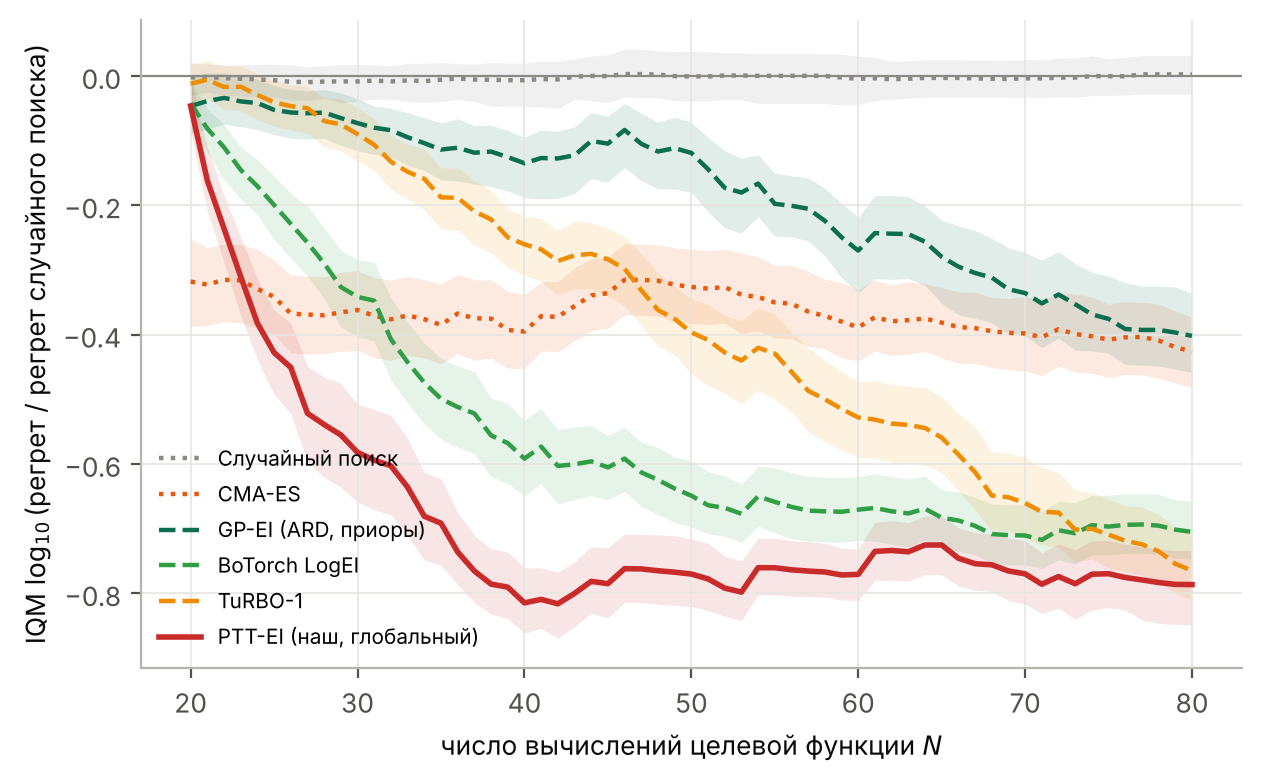
\includegraphics[width=0.49\linewidth]{e9_anytime.png}\hfill
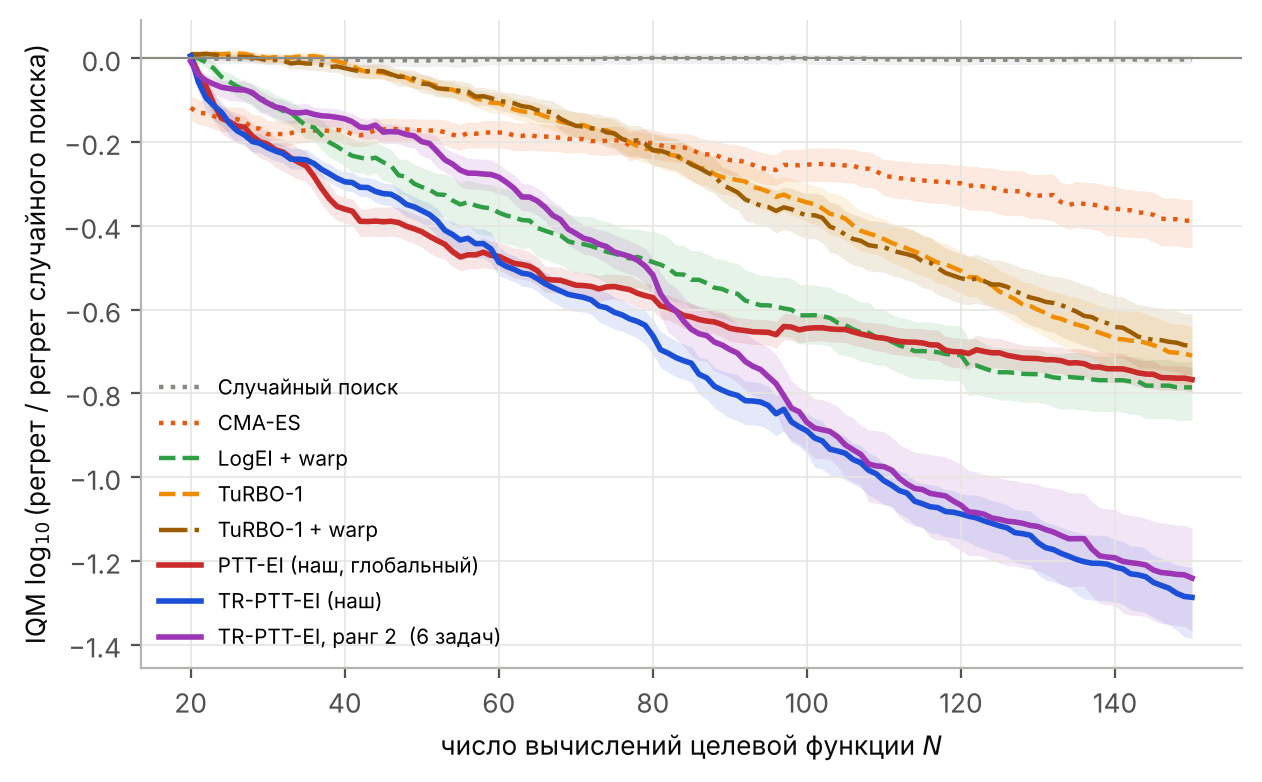
\includegraphics[width=0.49\linewidth]{e14_anytime.png}
\caption{Сводная оценка $S_N$~\eqref{eq:score} в зависимости от числа вычислений $N$ (меньше~--- лучше,
полоса~--- 95\% бутстреп-интервал). Слева: базовый эксперимент E9 (11~задач, $d=6$--$12$). Справа:
отложенные задачи E14 (9~задач, $d=10$--$20$).}\label{fig:main}
\end{figure}

\begin{table}[t]
\centering\small
\caption{Базовый эксперимент E9: $S_N$ и 95\% интервал (11~задач $\times$ 10~сидов)}\label{tab:e9}
\begin{tabular}{lcc}
\toprule
Метод & $N=40$ & $N=100$ \\
\midrule
PTT-EI (предлагаемый) & $\mathbf{-0.82}$ $[-0.87,-0.77]$ & $-0.86$ $[-0.92,-0.81]$ \\
BoTorch LogEI & $-0.59$ $[-0.66,-0.53]$ & $-0.80$ $[-0.85,-0.76]$ \\
TuRBO-1 & $-0.26$ $[-0.31,-0.21]$ & $\mathbf{-0.98}$ $[-1.05,-0.91]$ \\
Аддитивный GP-EI & $-0.25$ $[-0.31,-0.19]$ & $-0.61$ $[-0.66,-0.55]$ \\
GP-EI (ARD, приоры) & $-0.14$ $[-0.19,-0.09]$ & $-0.56$ $[-0.60,-0.51]$ \\
CMA-ES & $-0.40$ $[-0.46,-0.34]$ & $-0.49$ $[-0.55,-0.43]$ \\
Случайный поиск & $\phantom{-}0.00$ & $\phantom{-}0.00$ \\
\bottomrule
\end{tabular}
\end{table}

\textbf{Результаты базового эксперимента.} На рис.~\ref{fig:main} (слева) видно, что кривая PTT-EI
опускается быстрее всех: после 40~вычислений она лучше всех методов и лучше по медиане на 10 из 11~задач
(табл.~\ref{tab:e9}); против TuRBO-1 PTT-EI выигрывает в 90 из 110 пар (задача, сид). Однако после ~40
вычислений доля шагов, улучшающих лучшее значение, падает с 17\% до 5\%, и к $N=100$ TuRBO-1 выходит вперёд.
PTT-EI значимо лучше нашего GP-EI с приорами (99 из 110 пар на $N=40$, 75 из 100 на $N=100$).

\textbf{Непротиворечивость.} Исходная гипотеза <<PTT выигрывает за счёт малого TT-ранга целевой функции>>
не подтвердилась: поворот делает TT-ранг Rosenbrock10 и Dixon-Price10 равным~21 (вместо 3), но регрет
PTT-EI почти не меняется, а ранговая корреляция выигрыша с рангом функции близка к нулю (Спирмен,
$\rho\approx0$). Абляции E10 показывают, что ранг $2/4/8$ и длина $\ell$ почти не влияют на результат,
а замена ANOVA-приора на нулевой увеличивает регрет в 2--4~раза. Значит, выигрыш даёт ANOVA-приор:
модель в первую очередь описывает однопеременные и парные эффекты, что полезно при малой выборке.

\textbf{Улучшение и проверка на отложенных задачах.} Эксперимент E13 (схема $2\times2$: глобальная или
локальная модель, исходный или преобразованный выход~\cite{cowenrivers2022hebo}) показал, что застревание
устраняет именно локальная модель в доверительной области; преобразование выхода поверх неё не помогает.
На отложенных задачах (рис.~\ref{fig:main}, справа) TR-PTT-EI достигает $S_N=-1.39$ $[-1.49,-1.30]$ против
$-0.80$ у TuRBO-1, $-0.77$ у TuRBO-1 с преобразованием выхода и $-0.82$ у LogEI с преобразованием выхода.
Все три гипотезы протокола подтверждены парным тестом Уилкоксона по 90~парам: H1~--- 75:15,
$p=2\cdot10^{-10}$; H2~--- 71:19, $p=2\cdot10^{-9}$; H3~--- 81:9, $p=2\cdot10^{-14}$. Вариант TR-PTT лучший
по медиане на всех 9~задачах. Ограничения: синтетические функции, $d\le20$, $N\le200$; при $d=10$ один прогон
TR-PTT в 1.7--3.6~раза дороже TuRBO-1 по времени; на Hartmann6 лучшим остаётся TuRBO-1.

%=====================================================================
\section{Заключение}
Вероятностный тензорный поезд с ANOVA-приором и лапласовской неопределённостью оказался эффективным
суррогатом для BO на малых бюджетах, а его локальная версия TR-PTT превзошла TuRBO-1 и LogEI на отложенных
задачах размерности 10--20. Дальнейшие шаги: реальные задачи (подбор гиперпараметров, оптимизация
молекулярных и кластерных конфигураций~\cite{sozykin2026clusters}), размерности $d\ge50$, дискретные и смешанные
переменные (где естественны TT-методы~\cite{ryzhakov2023constructive,batsheva2023protes}), ускорение
лапласовского прогноза.

\bibliographystyle{unsrt}
\bibliography{references}
\end{document}
